% EIP-3009 Payment Flow - Standalone TikZ
% Compile with: pdflatex eip3009-flow.tex

\documentclass[tikz,border=10pt]{standalone}
\usepackage{tikz}
\usetikzlibrary{arrows.meta, shapes.geometric, positioning, calc, fit}
\usepackage{xcolor}

% Define colors
\definecolor{t402blue}{HTML}{3B82F6}
\definecolor{t402green}{HTML}{10B981}
\definecolor{t402purple}{HTML}{8B5CF6}
\definecolor{t402gray}{HTML}{6B7280}
\definecolor{t402orange}{HTML}{F59E0B}

\begin{document}
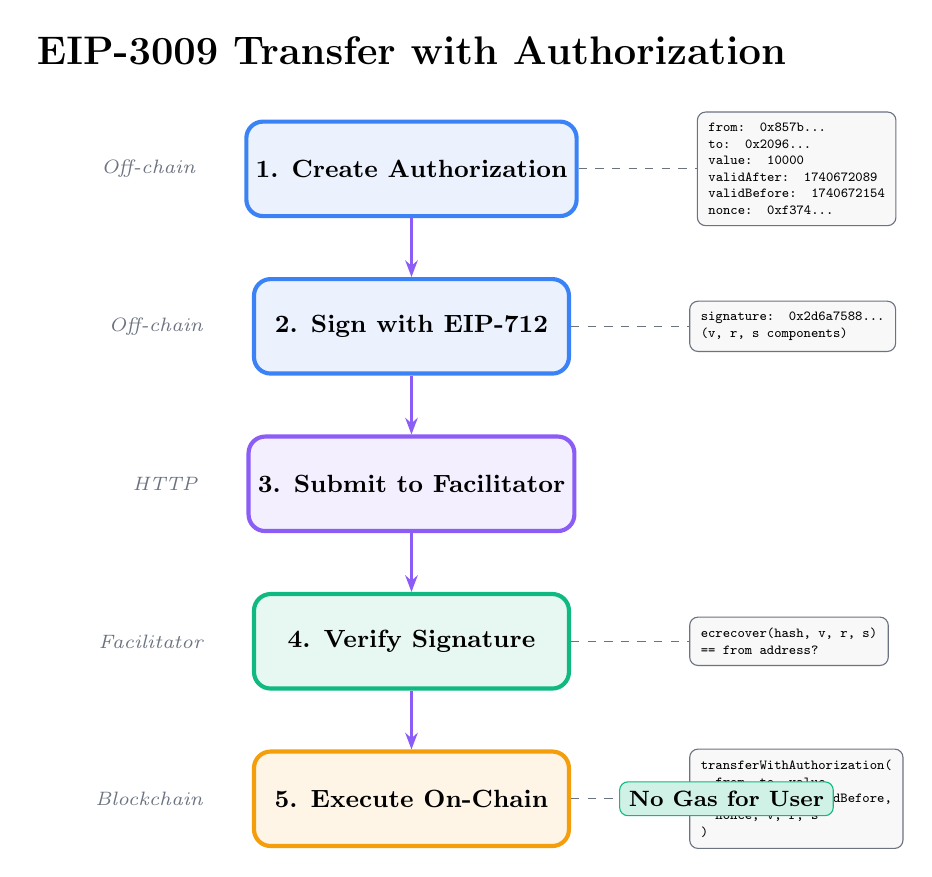
\begin{tikzpicture}[
    node distance=1.5cm,
    box/.style={
        rectangle,
        rounded corners=6pt,
        minimum width=4cm,
        minimum height=1.2cm,
        draw=#1,
        line width=1.5pt,
        fill=#1!10,
        font=\small\bfseries,
        align=center
    },
    arrow/.style={
        ->,
        >={Stealth[length=6pt]},
        line width=1.2pt,
        t402purple
    },
    label/.style={
        font=\footnotesize,
        fill=white,
        inner sep=2pt
    },
    data/.style={
        rectangle,
        rounded corners=3pt,
        draw=t402gray,
        fill=t402gray!5,
        font=\ttfamily\tiny,
        align=left,
        inner sep=4pt
    }
]

% Title
\node[font=\bfseries\Large] at (0,5) {EIP-3009 Transfer with Authorization};

% Flow boxes
\node[box=t402blue] (create) at (0,3.5) {1. Create Authorization};
\node[box=t402blue] (sign) at (0,1.5) {2. Sign with EIP-712};
\node[box=t402purple] (submit) at (0,-0.5) {3. Submit to Facilitator};
\node[box=t402green] (verify) at (0,-2.5) {4. Verify Signature};
\node[box=t402orange] (execute) at (0,-4.5) {5. Execute On-Chain};

% Data boxes
\node[data, right=1.5cm of create] (auth-data) {
from: 0x857b...\\
to: 0x2096...\\
value: 10000\\
validAfter: 1740672089\\
validBefore: 1740672154\\
nonce: 0xf374...
};

\node[data, right=1.5cm of sign] (sig-data) {
signature: 0x2d6a7588...\\
(v, r, s components)
};

\node[data, right=1.5cm of verify] (verify-data) {
ecrecover(hash, v, r, s)\\
== from address?
};

\node[data, right=1.5cm of execute] (tx-data) {
transferWithAuthorization(\\
\ \ from, to, value,\\
\ \ validAfter, validBefore,\\
\ \ nonce, v, r, s\\
)
};

% Arrows
\draw[arrow] (create) -- (sign);
\draw[arrow] (sign) -- (submit);
\draw[arrow] (submit) -- (verify);
\draw[arrow] (verify) -- (execute);

% Connect data boxes
\draw[t402gray, dashed] (create.east) -- (auth-data.west);
\draw[t402gray, dashed] (sign.east) -- (sig-data.west);
\draw[t402gray, dashed] (verify.east) -- (verify-data.west);
\draw[t402gray, dashed] (execute.east) -- (tx-data.west);

% Annotations
\node[font=\scriptsize\itshape, t402gray, left=0.5cm of create] {Off-chain};
\node[font=\scriptsize\itshape, t402gray, left=0.5cm of sign] {Off-chain};
\node[font=\scriptsize\itshape, t402gray, left=0.5cm of submit] {HTTP};
\node[font=\scriptsize\itshape, t402gray, left=0.5cm of verify] {Facilitator};
\node[font=\scriptsize\itshape, t402gray, left=0.5cm of execute] {Blockchain};

% Gas indicator
\node[rectangle, rounded corners=3pt, draw=t402green, fill=t402green!20, font=\footnotesize\bfseries] at (4,-4.5) {No Gas for User};

\end{tikzpicture}
\end{document}
